\documentclass[12pt, letterpaper, titlepage]{article}

\setlength\voffset{0pt}
\setlength\headsep{25pt}
\setlength\headheight{12pt}
\setlength\topmargin{0pt}
\addtolength\topmargin{-\headheight}
\addtolength\topmargin{-\headsep}
\setlength\hoffset{0pt}
\setlength\marginparwidth{0pt}
\setlength\oddsidemargin{0pt}
\setlength\textwidth{\paperwidth}
\addtolength\textwidth{-2in}
\setlength\textheight{\paperheight}
\addtolength\textheight{-2in}
\setlength{\parindent}{0pt}
\setlength{\parskip}{3pt}
\setlength{\textfloatsep}{10pt plus 2pt minus 4pt}

\usepackage{graphicx}
\usepackage[justification=centering]{caption}
\usepackage{mathptmx}
\usepackage{tabularx}
\usepackage{array}
\usepackage{float}
\usepackage{needspace}
\usepackage{placeins}
\usepackage{etoolbox}
\usepackage{amsmath}
\usepackage{amssymb}
\usepackage{subcaption}
\usepackage{booktabs}
\usepackage{natbib}
\usepackage{hyperref}
\usepackage{enumitem}

\setcounter{tocdepth}{2}

\pretocmd{\section}{\needspace{8\baselineskip}}{}{}
\pretocmd{\subsection}{\needspace{6\baselineskip}}{}{}
\clubpenalty=10000
\widowpenalty=10000
\displaywidowpenalty=10000

\newcommand{\TableHere}[1][0.34\textheight]{%
  \Needspace{#1}%
  \begin{table}[H]%
}
\newcommand{\FigureHere}[1][0.30\textheight]{%
  \Needspace{#1}%
  \begin{figure}[H]%
}

\newcommand{\tab}{\hspace*{2em}}
\newcolumntype{C}[1]{>{\centering\arraybackslash}p{#1}}
\newcolumntype{L}[1]{>{\raggedright\arraybackslash}p{#1}}
\newcolumntype{Y}{>{\raggedright\arraybackslash}X}

\bibliographystyle{plainnat}

%%%%%%%%%%%%%%%%%%%%%%%%%%%%%%%%%%%%%%%
\begin{document}
%%%%%%%%%%%%%%%%%%%%%%%%%%%%%%%%%%%%%%%

\title{Face Image Quality Prediction with a Compact CNN\\for Generative Training Support}
\author{Odon Ineza \\ Summer Research Project \\ Advisors: Spencer Giddens; Prof.\ Adam Czajka}
\date{\today}
\maketitle
\pagenumbering{roman}

\tableofcontents
\clearpage
\listoffigures
\clearpage
\listoftables
\clearpage
\pagenumbering{arabic}
\setcounter{page}{1}


\section{Introduction and Problem Statement}
\label{sec:intro}

Large generative models that synthesize or reconstruct face images are typically optimized with pixel-level reconstruction losses (e.g., $\ell_1$ or $\ell_2$), perceptual losses, and/or adversarial objectives \citep{goodfellow2014gan}. Those objectives encourage structural plausibility, but they do not by themselves guarantee that outputs are \emph{operationally usable}: images may remain blurry, poorly illuminated, awkwardly posed, compressed, or otherwise degraded in ways that matter for identity verification, biometric matching, and human review. The research need motivating this project is therefore a mechanism that can explicitly score whether a face image looks like a \emph{good, usable} sample along the quality dimensions encoded in an existing labeled dataset.

This work designs, implements, and trains a \textbf{small convolutional neural network (CNN)} that maps a single face image to a scalar quality score. The network is not intended as a standalone consumer product. It is intended as a learned approximation of an expensive algorithmic quality assessor---Open Source Face Image Quality (OFIQ) \citep{bsi2024ofiq,iso29794_5_2025}---so that quality can be estimated in milliseconds rather than seconds. In the broader research program, such a network is a natural candidate for later use as a differentiable quality critic inside a generative training loop. \textbf{That downstream wiring is treated in this report as an assumption about intended use (Section~\ref{sec:assumption}), not as completed engineering.}

The concrete deliverable of the present effort is therefore: (i)~a trained compact regressor on FFHQ faces labeled by OFIQ; (ii)~a defensible account of what ``quality'' means in this dataset; (iii)~architecture and loss choices matched to that definition; and (iv)~held-out evidence that predictions align with ground truth. The problem-statement rubric items addressed in depth are understanding the data, defining the task, designing a small CNN, and training/validating it (Sections~\ref{sec:data}--\ref{sec:results} and~\ref{sec:rubric}).

\section{Motivation and Research Context}
\label{sec:motivation}

\subsection{Why algorithmic face quality exists}

Face image quality assessment has a long history in biometrics because matching accuracy depends strongly on sample quality. OFIQ implements a unified quality score and a family of component measures aligned with ISO/IEC 29794-5 \citep{iso29794_5_2025,bsi2024ofiq}. Running OFIQ on tens of thousands of images is accurate but slow: on the order of seconds per image in our cluster jobs. A CNN that approximates the unified score enables large-scale scoring, rapid experimentation, and---under the assumption of Section~\ref{sec:assumption}---cheap quality feedback during generator training.

\subsection{Why a compact model is required}

If a quality network is ever evaluated repeatedly inside another model's training step, parameter count and inference cost matter as much as accuracy. The brief therefore emphasizes a \emph{small} CNN. We interpret ``small'' operationally as: substantially fewer parameters than a stock ResNet-18 \citep{he2016resnet}, trainable from scratch on offline compute nodes without ImageNet weight downloads \citep{deng2009imagenet,paszke2019pytorch}, and regularized aggressively enough to avoid memorizing 63{,}000 training faces.

\subsection{What this report contributes}

Relative to a typical ``train a classifier'' exercise, this report emphasizes:
\begin{enumerate}[leftmargin=*]
    \item an explicit definition of the ground-truth label (\texttt{UnifiedQualityScore.native});
    \item a regression formulation with ranking-aware loss;
    \item a custom SmallResNet ($\approx 0.33$M parameters) that replaced an overfit ResNet-18 baseline;
    \item measurement fixes requested by Spencer Giddens (checkpoint selection and clean train logging);
    \item quantitative held-out evaluation with MAE, Pearson $r$, Spearman $\rho$, and $R^2$.
\end{enumerate}

\FloatBarrier
\section{Understanding the Data}
\label{sec:data}

Rubric item~1 requires knowing exactly what is being predicted and how labels were generated before architecture or loss design. This section answers that requirement for the FFHQ--OFIQ corpus used in this project.

\subsection{Image corpus: FFHQ}

The image source is Flickr-Faces-HQ (FFHQ), a curated set of 70{,}000 high-quality face photographs introduced with StyleGAN \citep{karras2019stylegan}. In our working copy, images are stored as RGB PNG files under paths of the form \texttt{ffhq\_all/00000.png} \ldots\ \texttt{ffhq\_all/69999.png}. Source resolution in the training tree used for this project is $256\times 256$; the network consumes $224\times 224$ crops/resizes at train and evaluation time.

\subsection{Label source: OFIQ Unified Quality Score}

Labels were produced by running OFIQ over the FFHQ collection and writing results to \texttt{ffhq\_all\_results.csv} (semicolon-separated; 70{,}000 data rows; 57 columns). OFIQ emits both a unified quality score and many component measures (sharpness, pose, illumination, occlusion-related quantities, etc.), each typically available in \texttt{.native} and \texttt{.scalar} forms \citep{bsi2024ofiq}.

The supervised target used throughout training and evaluation is:
\begin{center}
\textbf{\texttt{UnifiedQualityScore.native}}
\end{center}
Empirical range on the full CSV is approximately $[11.211,\,33.278]$. The companion column \texttt{UnifiedQualityScore.scalar} remaps quality onto a squashed display-oriented range (observed roughly $[1,98]$). We deliberately avoid the scalar target: nonlinear squashing distorts distances and makes absolute errors harder to interpret. Training on the native score keeps the regression target closer to the quantity OFIQ computes internally and yields errors that are directly readable in native units.

\FigureHere[0.38\textheight]
\centering
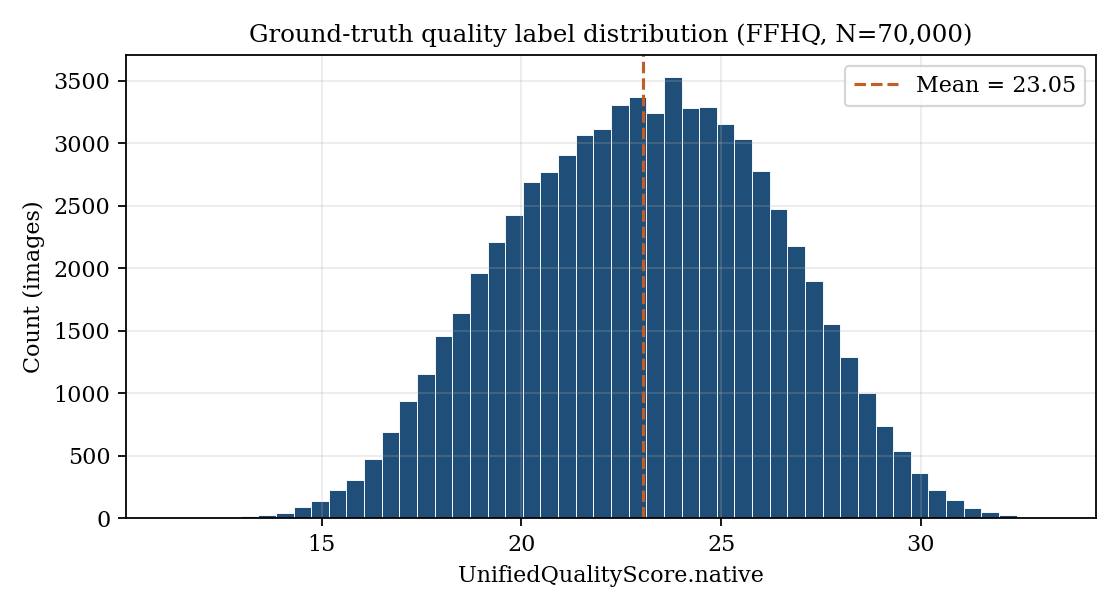
\includegraphics[width=0.92\textwidth]{figures/fig_label_histogram.png}
\caption{Histogram of \texttt{UnifiedQualityScore.native} over all 70{,}000 labeled FFHQ images. The distribution is unimodal and concentrated in the mid-twenties, with a usable dynamic range of roughly 22 native score points.}
\label{fig:label_hist}
\end{figure}

\subsection{Joining labels to pixels}

Each CSV row is joined to its image \textbf{by filename}, never by row order. The training script filters to rows whose image file exists on disk and whose target is finite. A historical missing-file list (\texttt{ffhq\_MISSING\_list.txt}, 21{,}877 names) documents an earlier incomplete local copy; the full training run used for the results in this report reported 70{,}000 usable labeled images after filtering.

\subsection{Train / validation split}

After filtering, we randomly permute indices with seed~42 and hold out 10\%:
\begin{itemize}[leftmargin=*]
    \item Training set: 63{,}000 images (90\%);
    \item Held-out validation / test set: 7{,}000 images (10\%).
\end{itemize}
Validation filenames are written to \texttt{best\_model\_full.val\_files.txt} so later evaluation cannot silently reconstruct a different split. Target min--max scaling uses \textbf{training-set statistics only} (with a 5\% margin), preventing leakage of validation extrema into the scaled loss.

\TableHere[10\baselineskip]
\caption{Dataset summary used for supervised quality regression.}
\label{tab:dataset}
\centering
\footnotesize
\begin{tabularx}{\textwidth}{|L{0.34\textwidth}|Y|}
\hline
\textbf{Property} & \textbf{Value} \\
\hline
Image source & FFHQ, 70{,}000 faces \citep{karras2019stylegan} \\
\hline
Working resolution & $256\times 256$ PNG RGB; model input $224\times 224$ \\
\hline
Label file & \texttt{ffhq\_all\_results.csv} (OFIQ) \\
\hline
Target column & \texttt{UnifiedQualityScore.native} \\
\hline
Native score range (full set) & $\approx 11.21$ -- $33.28$ \\
\hline
Train / val sizes & 63{,}000 / 7{,}000 (seed 42, 10\% holdout) \\
\hline
Join key & \texttt{Filename} \\
\hline
\end{tabularx}
\end{table}

\subsection{What ``quality'' means in this project}

In this dataset, quality is \textbf{not} a human Likert annotation collected for this study. It is an \textbf{algorithmic unified score} produced by OFIQ, which aggregates multiple biometric quality factors into one scalar \citep{bsi2024ofiq,iso29794_5_2025}. Component columns exist and could support multi-head prediction in future work; the present model predicts only the unified native score. That choice matches the problem statement's ``scalar (or low-dimensional)'' language while keeping the first deliverable focused and evaluable.

\FloatBarrier
\section{Task Definition}
\label{sec:task}

Rubric item~2 requires a precise task definition because it determines the output layer, loss, and success metrics.

\subsection{Problem type: supervised regression}

We formulate face image quality prediction as supervised regression:
\begin{align}
x &\in \mathbb{R}^{3\times 224\times 224}, \\
y &\in \mathbb{R}, \quad y = \texttt{UnifiedQualityScore.native}(x), \\
f_\theta(x) &\approx y.
\end{align}
The network emits a single continuous value. We do \textbf{not} discretize quality into buckets (classification), because the ground truth is continuous and ranking fidelity matters for downstream use.

\subsection{Output representation and scaling}

Internally, targets are min--max scaled to $[0,1]$ using training-set bounds $(y_{\mathrm{lo}}, y_{\mathrm{hi}})$. The network head ends in a sigmoid so predictions $\hat{z}\in(0,1)$ match that scaled space. Native-unit predictions are recovered by
\begin{equation}
\hat{y} = \hat{z}\,(y_{\mathrm{hi}}-y_{\mathrm{lo}}) + y_{\mathrm{lo}}.
\label{eq:unscale}
\end{equation}
Checkpoint metadata stores $y_{\mathrm{lo}}$, $y_{\mathrm{hi}}$, architecture name, image size, and training epoch so inference is reproducible.

\subsection{Loss function matched to the task}

Pure mean squared error (MSE) penalizes absolute deviation but does not directly optimize ranking correlation---yet Pearson $r$ and Spearman $\rho$ are the natural success criteria for a quality scorer \citep{pearson1896correlation,spearman1904correlation}. We therefore use a combined loss
\begin{equation}
\mathcal{L} = 0.6\,\mathrm{MSE}(\hat{z}, z) + 0.4\bigl(1 - r_{\mathrm{Pearson}}(\hat{z}, z)\bigr),
\label{eq:loss}
\end{equation}
where $z$ is the scaled target. The Pearson term supplies gradient signal toward correct ordering of images by quality.

\subsection{Evaluation metrics}

Held-out success is reported in native units where possible:
\begin{itemize}[leftmargin=*]
    \item \textbf{MAE / RMSE:} absolute accuracy;
    \item \textbf{Pearson $r$:} linear agreement with OFIQ;
    \item \textbf{Spearman $\rho$:} rank agreement (primary quality-ranking metric);
    \item \textbf{$R^2$:} variance explained;
    \item \textbf{Baseline MAE:} error of always predicting the training-set mean (sanity check).
\end{itemize}

\TableHere[8\baselineskip]
\caption{Task definition summary.}
\label{tab:task}
\centering
\footnotesize
\begin{tabularx}{\textwidth}{|L{0.28\textwidth}|Y|}
\hline
\textbf{Aspect} & \textbf{Choice} \\
\hline
Learning problem & Supervised regression (not classification) \\
\hline
Output & Single scalar quality score \\
\hline
Ground truth & OFIQ \texttt{UnifiedQualityScore.native} \\
\hline
Training loss & $0.6\,\mathrm{MSE} + 0.4\,(1-r)$ \\
\hline
Primary eval metrics & MAE, Pearson $r$, Spearman $\rho$ \\
\hline
Higher score means & Higher predicted OFIQ unified quality \\
\hline
\end{tabularx}
\end{table}


\FloatBarrier
\section{Model Architecture: SmallResNet}
\label{sec:arch}

Rubric item~3 asks for a small CNN appropriate to the task size. We first tried a stock ResNet-18 and then replaced it with a custom compact residual network.

\subsection{Failure of ResNet-18 as a baseline}

ResNet-18 from \texttt{torchvision} has on the order of 11~million parameters and is commonly initialized from ImageNet weights \citep{he2016resnet,deng2009imagenet,paszke2019pytorch}. On this quality-regression task, that capacity produced catastrophic overfitting in earlier runs: training MAE near $1.7$ while validation MAE remained near $8.7$, with a validation/training MSE ratio of approximately $27\times$. The model memorized training faces and failed to generalize. Advisor guidance was to use the smallest ResNet that could still learn the mapping.

\subsection{SmallResNet design}

We built \texttt{SmallResNet} from scratch (no pretrained weights), with channel widths $(16,32,64,128)$ and \textbf{one} residual block per stage. Runtime parameter count is approximately \textbf{0.33~million}---roughly $30\times$ smaller than ResNet-18.

\FigureHere[0.28\textheight]
\centering
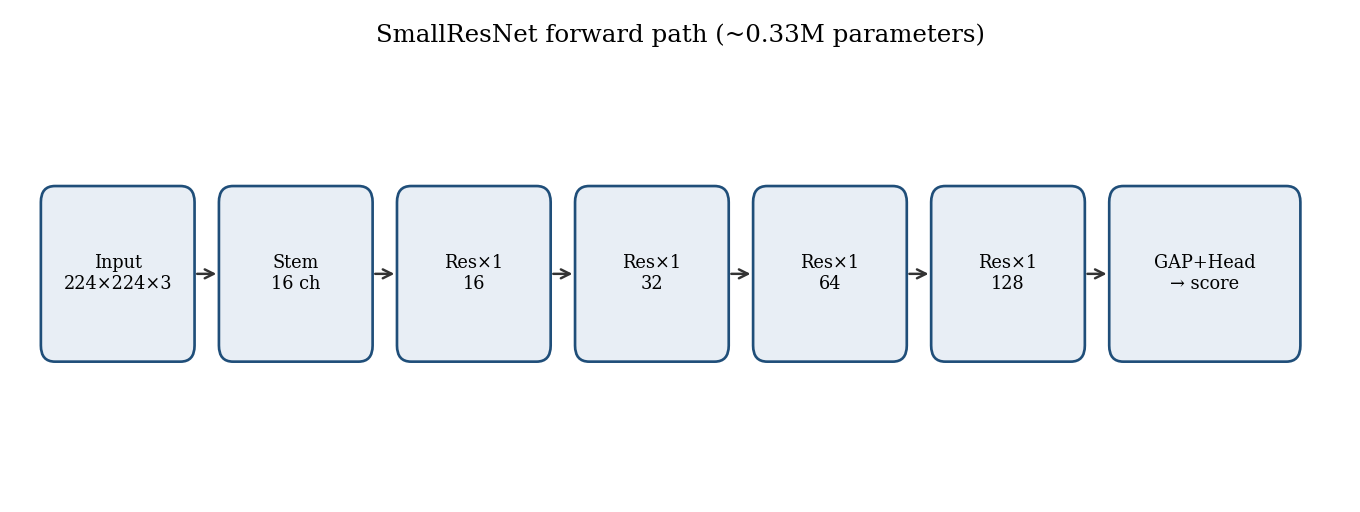
\includegraphics[width=0.98\textwidth]{figures/fig_architecture_schematic.png}
\caption{Forward path of SmallResNet: stem, four residual stages, global average pooling, and a two-layer regression head with sigmoid output in scaled $[0,1]$ space.}
\label{fig:arch}
\end{figure}

\TableHere[14\baselineskip]
\caption{SmallResNet layer progression for a $224\times 224$ RGB input.}
\label{tab:layers}
\centering
\footnotesize
\begin{tabularx}{\textwidth}{|L{0.30\textwidth}|C{0.22\textwidth}|Y|}
\hline
\textbf{Stage} & \textbf{Output shape} & \textbf{Notes} \\
\hline
Input & $224\times 224\times 3$ & Normalize with mean/std $0.5$ \\
\hline
Stem: Conv $3\times 3$, stride~2 + BN + ReLU & $112\times 112\times 16$ & \\
\hline
MaxPool $2\times 2$ & $56\times 56\times 16$ & \\
\hline
Residual block (stride~1) & $56\times 56\times 16$ & Dropout2d $0.10$ + SE \\
\hline
Residual block (stride~2) & $28\times 28\times 32$ & Dropout2d $0.10$ + SE \\
\hline
Residual block (stride~2) & $14\times 14\times 64$ & Dropout2d $0.10$ + SE \\
\hline
Residual block (stride~2) & $7\times 7\times 128$ & Dropout2d $0.10$ + SE \\
\hline
Global average pool & $128$ & \\
\hline
Dropout $0.30$ $\rightarrow$ Linear $128\to 64$ $\rightarrow$ ReLU & $64$ & \\
\hline
Dropout $0.30$ $\rightarrow$ Linear $64\to 1$ $\rightarrow$ Sigmoid & $1$ & Scaled quality \\
\hline
\end{tabularx}
\end{table}

Each residual block contains two $3\times 3$ convolutions with batch normalization, a spatial dropout layer \citep{tompson2015spatialDropout}, a Squeeze-and-Excitation (SE) module with reduction ratio~4 \citep{hu2018senet}, and a shortcut connection \citep{he2016resnet}. SE reweights channels so the network can emphasize quality-relevant feature maps (e.g., sharpness- or illumination-related activations) with negligible parameter cost.

\FigureHere[0.36\textheight]
\centering
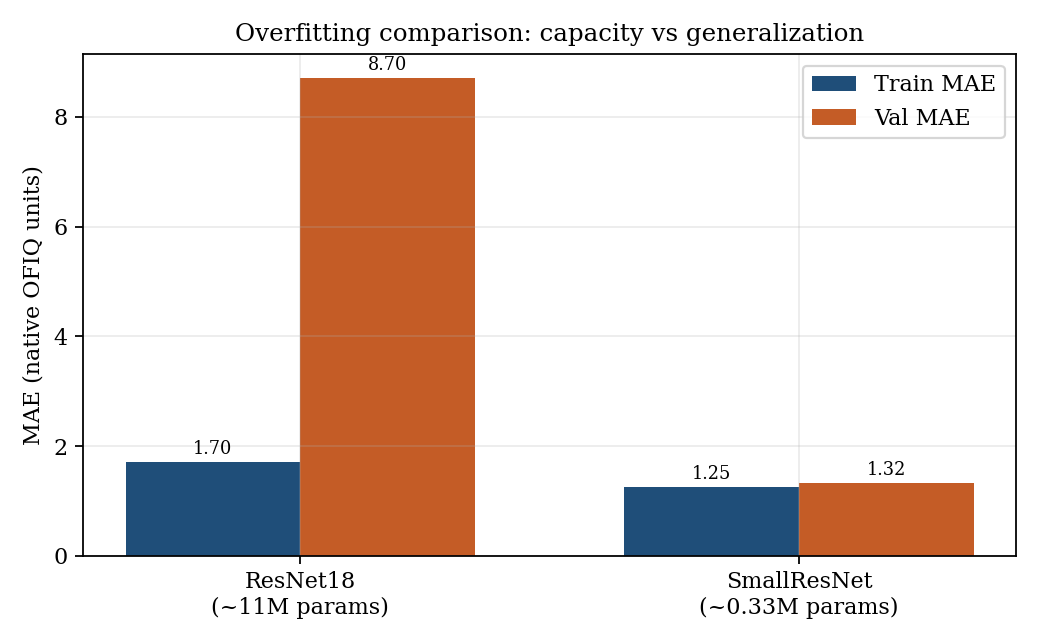
\includegraphics[width=0.78\textwidth]{figures/fig_overfit_comparison.png}
\caption{Train versus validation MAE for ResNet-18 (earlier overfit baseline) and SmallResNet (final model). Reducing capacity collapses the generalization gap.}
\label{fig:overfit_bar}
\end{figure}

\FloatBarrier
\section{Anti-Overfitting Design}
\label{sec:regularization}

Overfitting was the primary failure mode of the large baseline and a stated concern in advisor feedback. The following techniques were all implemented in \texttt{train\_quality.py}.

\subsection{Capacity control}
Using $\approx 0.33$M parameters instead of $\approx 11$M removes the ability to memorize 63{,}000 training images while still fitting a smooth quality function.

\subsection{Spatial dropout and head dropout}
Spatial dropout zeros entire feature maps with probability $0.10$ inside every residual block \citep{tompson2015spatialDropout}. Because neighboring activations in a conv map are correlated, dropping whole channels is more effective than elementwise dropout in convolutional trunks \citep{srivastava2014dropout}. The regression head additionally uses dropout probability $0.30$.

\subsection{Weight decay via AdamW}
Optimization uses AdamW with weight decay $1\times 10^{-4}$ \citep{loshchilov2019adamw}, decoupling $\ell_2$ regularization from the adaptive gradient update.

\subsection{Strong data augmentation}
During the weight-update pass, each training image is randomly transformed with RandomResizedCrop (scale $0.8$--$1.0$), horizontal flip, color jitter, and rotation of $\pm 10^\circ$. Evaluation and the clean logging pass use deterministic resize only.

\subsection{Combined MSE + Pearson loss}
Equation~\eqref{eq:loss} directly pressures ranking fidelity, which is the operational meaning of a quality score.

\subsection{Early stopping, LR scheduling, and gradient clipping}
Training monitors validation MSE with patience~8. Learning rate starts at $1\times 10^{-3}$ and is halved by ReduceLROnPlateau after 3 epochs without improvement. Gradients are clipped to max-norm $1.0$ to avoid the instability observed in earlier runs (validation MAE spike near epoch~8 before clipping was enabled).

\TableHere[12\baselineskip]
\caption{Regularization and training-stability controls.}
\label{tab:reg}
\centering
\footnotesize
\begin{tabularx}{\textwidth}{|L{0.30\textwidth}|Y|}
\hline
\textbf{Technique} & \textbf{Setting / role} \\
\hline
Small capacity & $\approx 0.33$M params \\
\hline
Dropout2d & $p=0.10$ in every residual block \\
\hline
Head dropout & $p=0.30$ (twice) \\
\hline
AdamW weight decay & $1\times 10^{-4}$ \\
\hline
SE attention & reduction 4 in every block \\
\hline
Augmentation & strong crop/flip/jitter/rotation \\
\hline
Loss & $0.6$ MSE + $0.4$ Pearson term \\
\hline
Early stopping & patience 8 on val MSE \\
\hline
Grad clip & max-norm $1.0$ \\
\hline
LR schedule & ReduceLROnPlateau, factor $0.5$, patience 3 \\
\hline
\end{tabularx}
\end{table}

\FloatBarrier
\section{Training Protocol}
\label{sec:train}

\subsection{Optimization setup}

Training ran on a single NVIDIA A10 GPU under PyTorch 2.9.1 with batch size~64 and 8 data-loader workers. Requested length was 40~epochs; early stopping did not trigger, so all 40~epochs completed. Wall-clock time was approximately 112--143~seconds per epoch ($\approx 75$~minutes total) after the clean-logging pass was added.

\subsection{Checkpoint selection (Spencer feedback)}

Originally, \texttt{best\_model\_full.pt} was overwritten whenever validation MSE reached a new low, so the saved weights came from epoch~37 rather than the last trained epoch. Spencer Giddens requested a simpler rule: \textbf{always keep the final epoch}. Early stopping still uses validation MSE to decide \emph{when} to stop; it no longer decides \emph{which} weights are delivered. The quality difference between epoch~37 and epoch~40 is negligible (val MAE $1.30$ vs.\ $1.32$).

\subsection{Clean train-metric logging (Spencer feedback)}

The original training curve measured ``train'' error during the dropout-on, augmented update pass, while validation used dropout-off deterministic transforms. That made train MAE appear \emph{worse} than val MAE for most of training---an artifact of measurement, not of generalization. The fix adds a second, dropout-off, non-augmented forward pass over the training set each epoch \textbf{for logging only}. Weight updates still use dropout and augmentation.

Table~\ref{tab:dropout_logging} makes the artifact concrete by comparing, at matched epochs, the metric each protocol reports. For both the train and the validation MAE, the gap column is \textbf{dropout-on value $-$ dropout-off value}: how much the measurement itself changes when dropout and augmentation are active during logging. The two columns play different roles. Validation MAE was measured dropout-off in \emph{both} runs, so its gap contains no dropout effect at all---it is a control that shows only the run-to-run drift between the two trainings ($-0.13$ to $+0.07$ after warm-up). The train MAE gap contains that same drift \emph{plus} the measurement artifact. The excess of the train gap over the validation gap therefore isolates what dropout and augmentation add to the measured train error: consistently about $+0.1$ score points at every epoch shown ($+0.09$, $+0.04$, $+0.13$, $+0.12$, $+0.14$, $+0.11$ at epochs 1--40). That systematic inflation, small as it looks, was enough to lift the reported train MAE above the val MAE and invert the expected shape of the training curves; the sources are spatial dropout ($p=0.10$ per block) and head dropout ($p=0.30$) perturbing the forward pass, and random crops, flips, rotations, and color jitter making the logged training images harder than their deterministic validation counterparts.

\TableHere[0.34\textheight]
\centering
\caption{What the logging protocol adds to each measured metric. Gap $=$ dropout-on value $-$ dropout-off value (native OFIQ units). Validation was measured dropout-off in both runs, so its gap reflects only run-to-run drift; the train gap additionally contains the dropout/augmentation measurement artifact.}
\label{tab:dropout_logging}
\small
\begin{tabular}{@{}c ccc ccc@{}}
\toprule
& \multicolumn{3}{c}{\textbf{Train MAE}} & \multicolumn{3}{c}{\textbf{Val MAE}} \\
\cmidrule(lr){2-4} \cmidrule(lr){5-7}
Epoch & Dropout on & Dropout off & Gap & Dropout on\textsuperscript{*} & Dropout off & Gap \\
\midrule
1  & 2.39 & 1.92 & $+0.47$ & 2.31 & 1.93 & $+0.38$ \\
5  & 1.65 & 1.54 & $+0.11$ & 1.64 & 1.56 & $+0.07$ \\
10 & 1.52 & 1.46 & $+0.06$ & 1.42 & 1.49 & $-0.07$ \\
20 & 1.44 & 1.44 & $-0.01$ & 1.36 & 1.49 & $-0.13$ \\
30 & 1.39 & 1.26 & $+0.13$ & 1.32 & 1.33 & $-0.01$ \\
40 & 1.37 & 1.25 & $+0.12$ & 1.33 & 1.32 & $+0.01$ \\
\bottomrule
\end{tabular}

\vspace{2pt}
{\footnotesize \textsuperscript{*}``Dropout on'' labels the archived \emph{run} whose train metric was logged with dropout and augmentation active; its validation metric was still measured dropout-off, which is why the val gap shows only run-to-run drift.}
\end{table}

\FigureHere[0.40\textheight]
\centering
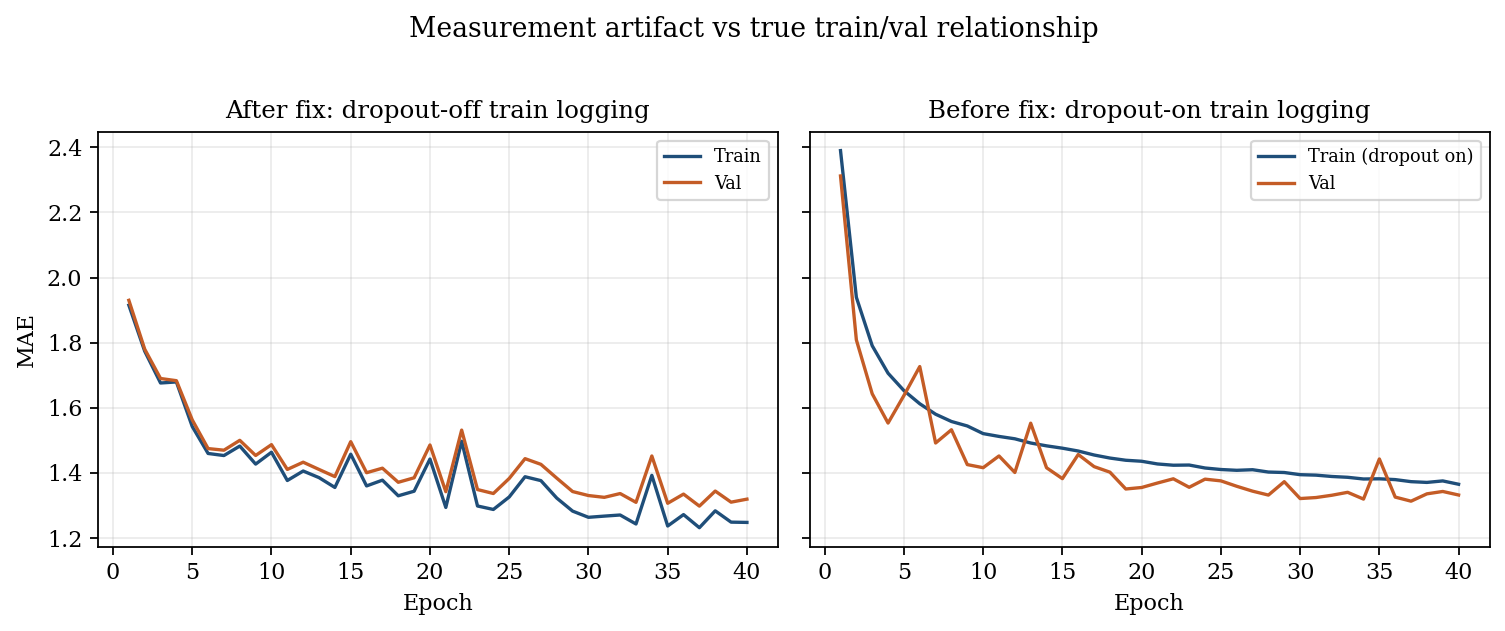
\includegraphics[width=0.98\textwidth]{figures/fig_logging_artifact.png}
\caption{Left: after the logging fix, train MAE lies below val MAE at every epoch. Right: archived curve from dropout-on train logging, which inverted the expected relationship.}
\label{fig:logging}
\end{figure}

\FigureHere[0.36\textheight]
\centering
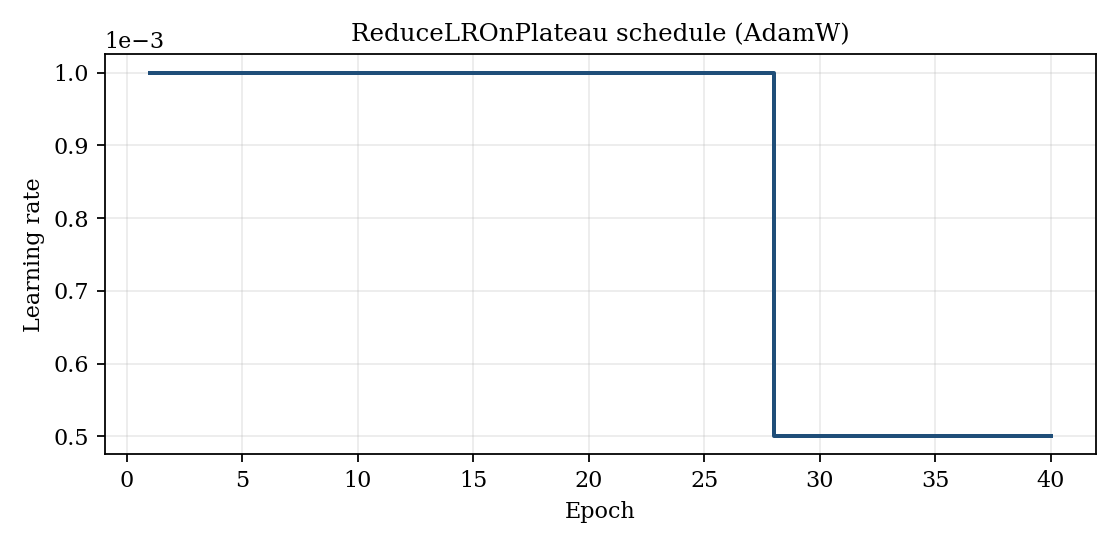
\includegraphics[width=0.92\textwidth]{figures/fig_lr_schedule.png}
\caption{Learning-rate schedule observed in the final 40-epoch run (ReduceLROnPlateau on AdamW).}
\label{fig:lr}
\end{figure}

\FloatBarrier
\section{Problems Encountered and Resolutions}
\label{sec:problems}

\TableHere[0.42\textheight]
\caption{Major issues encountered during development and how they were resolved.}
\label{tab:problems}
\centering
\footnotesize
\begin{tabularx}{\textwidth}{|L{0.28\textwidth}|Y|Y|}
\hline
\textbf{Problem} & \textbf{Evidence} & \textbf{Resolution} \\
\hline
ResNet-18 memorization & Val MAE $\approx 8.7$ vs train $\approx 1.7$; MSE ratio $\approx 27\times$ & Replace with SmallResNet ($\approx 0.33$M) + full regularization stack \\
\hline
Inverted train/val curves & Train MAE $>$ val MAE for most epochs & Second dropout-off logging pass; archive old curve for comparison \\
\hline
Ambiguous checkpoint & Saved epoch~37 (best val MSE) while training continued to~40 & Always save final epoch; mark best-val epoch as reference only \\
\hline
Gradient spike (earlier) & Val MAE jump $\sim 17\to 23$ near epoch~8 & Gradient clipping at max-norm $1.0$ \\
\hline
Scalar vs native target & Scalar squashing distorts regression geometry & Train on \texttt{UnifiedQualityScore.native} only \\
\hline
Incomplete local images & \texttt{ffhq\_MISSING\_list.txt} (21{,}877 names) & Filter by file existence; full run used 70{,}000 usable rows \\
\hline
\end{tabularx}
\end{table}

These resolutions are not cosmetic. The ResNet-18 failure showed that architecture choice dominates generalization on this dataset. The logging fix changed how we \emph{diagnose} overfitting without changing the optimizer's update rule. The checkpoint rule change made the delivered artifact match the narrative of ``the model we finished training.''


\FloatBarrier
\section{Results and Evaluation}
\label{sec:results}

Rubric item~4 requires proper splitting, an appropriate loss, and evidence that predictions correlate with ground truth. All metrics below use the held-out 7{,}000-image list unless noted.

\subsection{Training progression}

Table~\ref{tab:epochs} summarizes selected epochs from \texttt{train\_log\_full.csv}. Train and validation MAE are both measured with dropout off and without augmentation, so the gap is interpretable.

\TableHere[12\baselineskip]
\caption{Selected epochs from the final clean-logging run. Epoch~40 is the saved checkpoint; epoch~37 had the lowest validation MSE (reference only).}
\label{tab:epochs}
\centering
\footnotesize
\begin{tabularx}{\textwidth}{|C{0.10\textwidth}|C{0.14\textwidth}|C{0.14\textwidth}|C{0.16\textwidth}|C{0.14\textwidth}|Y|}
\hline
\textbf{Epoch} & \textbf{Train MAE} & \textbf{Val MAE} & \textbf{Gap (val$-$train)} & \textbf{Val MSE} & \textbf{Notes} \\
\hline
1 & 1.92 & 1.93 & $+0.01$ & 0.01009 & start \\
\hline
5 & 1.54 & 1.56 & $+0.02$ & 0.00661 & \\
\hline
10 & 1.46 & 1.49 & $+0.02$ & 0.00597 & \\
\hline
20 & 1.44 & 1.49 & $+0.04$ & 0.00593 & \\
\hline
30 & 1.26 & 1.33 & $+0.07$ & 0.00479 & \\
\hline
37 & 1.23 & 1.30 & $+0.07$ & 0.00461 & lowest val MSE \\
\hline
\textbf{40} & \textbf{1.25} & \textbf{1.32} & $\mathbf{+0.07}$ & \textbf{0.00474} & \textbf{saved} \\
\hline
\end{tabularx}
\end{table}

\FigureHere[0.38\textheight]
\centering
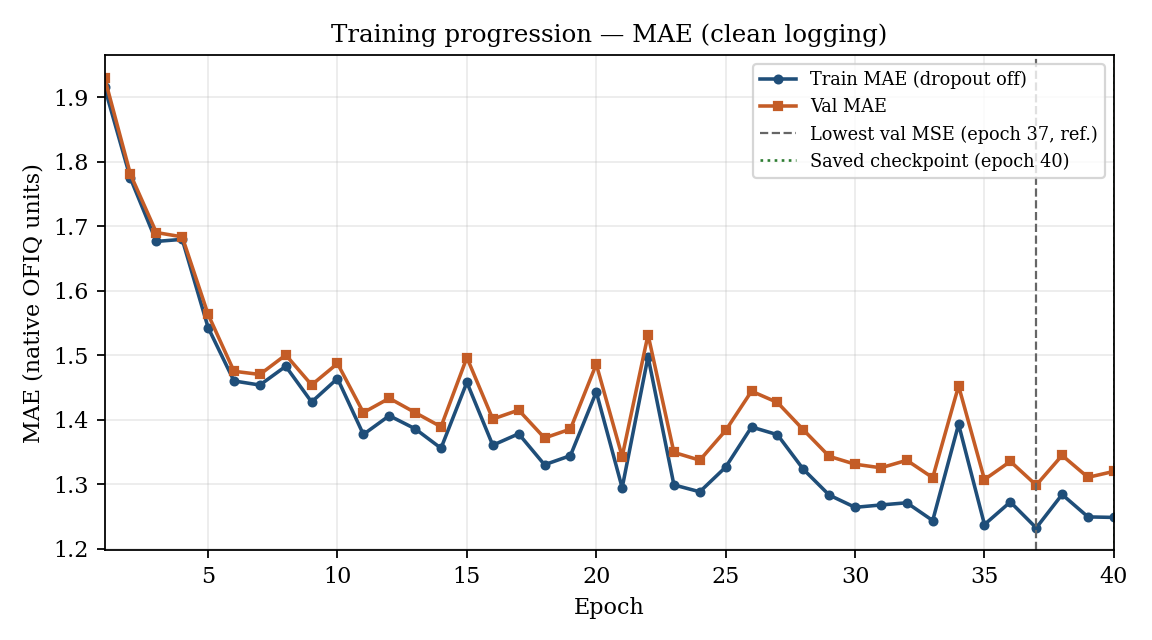
\includegraphics[width=0.92\textwidth]{figures/fig_train_val_mae.png}
\caption{Train and validation MAE across 40 epochs under clean logging. The dashed line marks the lowest-val-MSE epoch (reference); the dotted line marks the saved final checkpoint.}
\label{fig:mae_curve}
\end{figure}

\FigureHere[0.36\textheight]
\centering
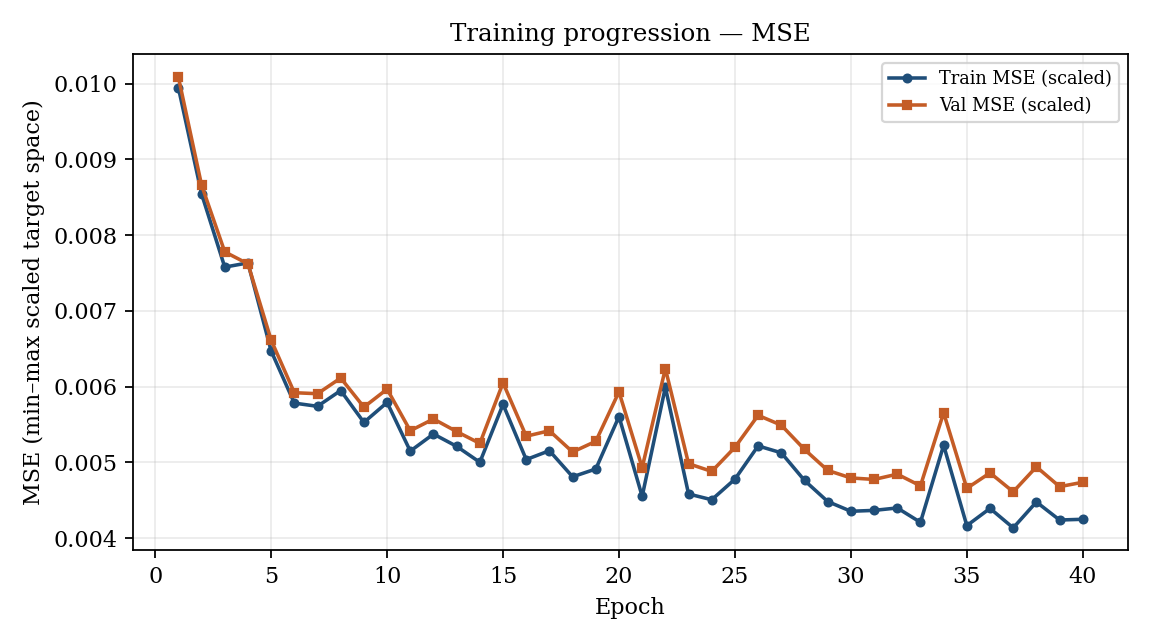
\includegraphics[width=0.92\textwidth]{figures/fig_train_val_mse.png}
\caption{Train and validation MSE in scaled target space. Curves remain close throughout training (ratio $\approx 1.1\times$ at the end).}
\label{fig:mse_curve}
\end{figure}

\FigureHere[0.40\textheight]
\centering

\includegraphics[width=0.92\textwidth]{figures/train_curve_full.png}
\caption{Full training-curve artifact produced by \texttt{train\_quality.py} (\texttt{train\_curve\_full.png}).}
\label{fig:train_curve_full}
\end{figure}

\subsection{Overfitting check}

At the saved epoch, the validation/training MSE ratio is approximately $1.1\times$, versus $\approx 27\times$ for the ResNet-18 baseline. The train/val MAE gap is only $+0.07$ native score points. Automated diagnosis flags a mild uptick in validation loss after epoch~37; that movement is within early-stopping patience and does not indicate memorization.

\subsection{Held-out metrics}

Evaluating \texttt{best\_model\_full.pt} (epoch~40) on the 7{,}000 held-out images yields:

\TableHere[10\baselineskip]
\caption{Held-out evaluation on 7{,}000 images never used for gradient updates.}
\label{tab:heldout}
\centering
\footnotesize
\begin{tabularx}{\textwidth}{|L{0.28\textwidth}|C{0.16\textwidth}|Y|}
\hline
\textbf{Metric} & \textbf{Value} & \textbf{Interpretation} \\
\hline
MAE & \textbf{1.32} & Mean absolute error in native OFIQ units \\
\hline
Baseline MAE & 2.68 & Always predict mean score \\
\hline
RMSE & 1.67 & Emphasizes larger mistakes \\
\hline
Pearson $r$ & \textbf{0.866} & Strong linear correlation \\
\hline
Spearman $\rho$ & \textbf{0.867} & Strong rank agreement \\
\hline
$R^2$ & 0.738 & 73.8\% of variance explained \\
\hline
\end{tabularx}
\end{table}

\FigureHere[0.34\textheight]
\centering
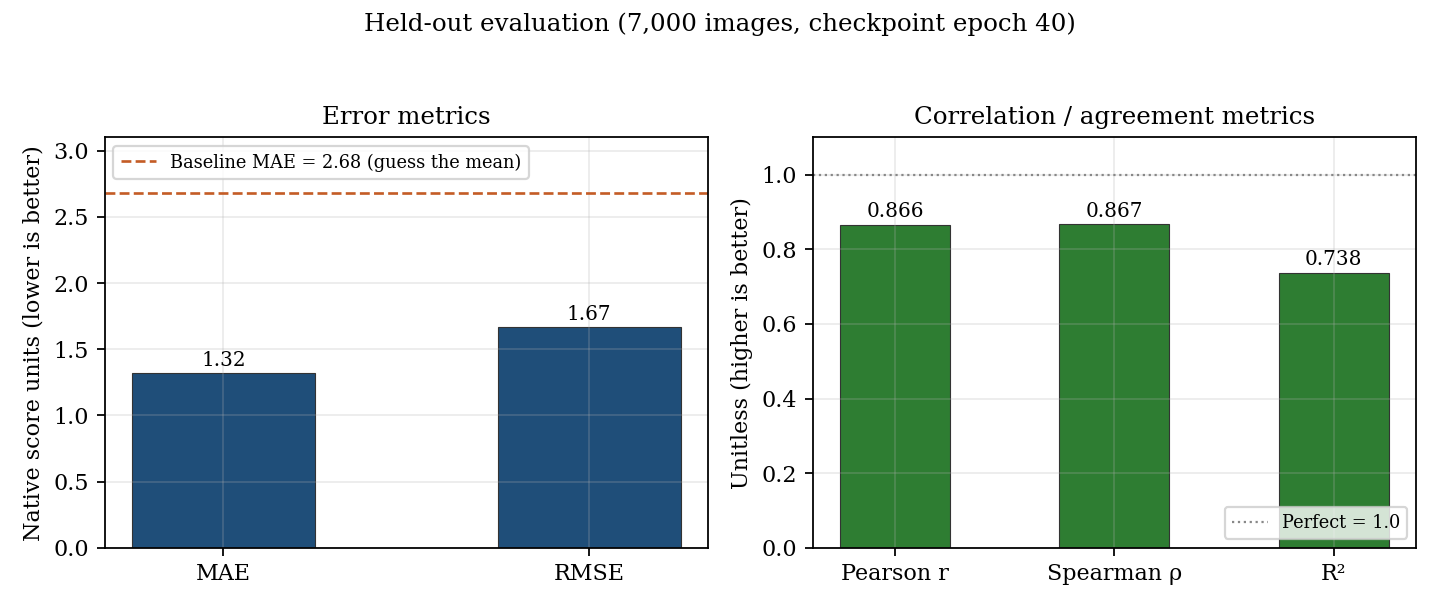
\includegraphics[width=0.88\textwidth]{figures/fig_metrics_summary.png}
\caption{Summary of held-out metrics relative to the mean-predictor baseline MAE.}
\label{fig:metrics_bar}
\end{figure}

On a native score span of roughly 22 points, MAE $1.32$ is about 6\% relative error. Beating the baseline by roughly $2\times$ confirms that the network uses image content rather than predicting a constant.

\FigureHere[0.42\textheight]
\centering
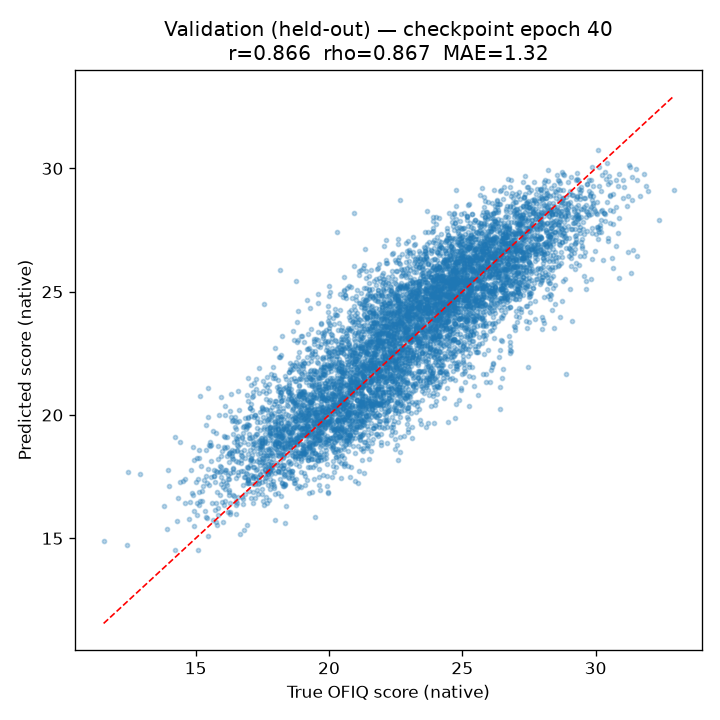
\includegraphics[width=0.88\textwidth]{figures/eval_scatter_full.png}
\caption{Predicted versus true native scores on the held-out validation set (7{,}000 images).}
\label{fig:scatter_val}
\end{figure}

\FigureHere[0.42\textheight]
\centering
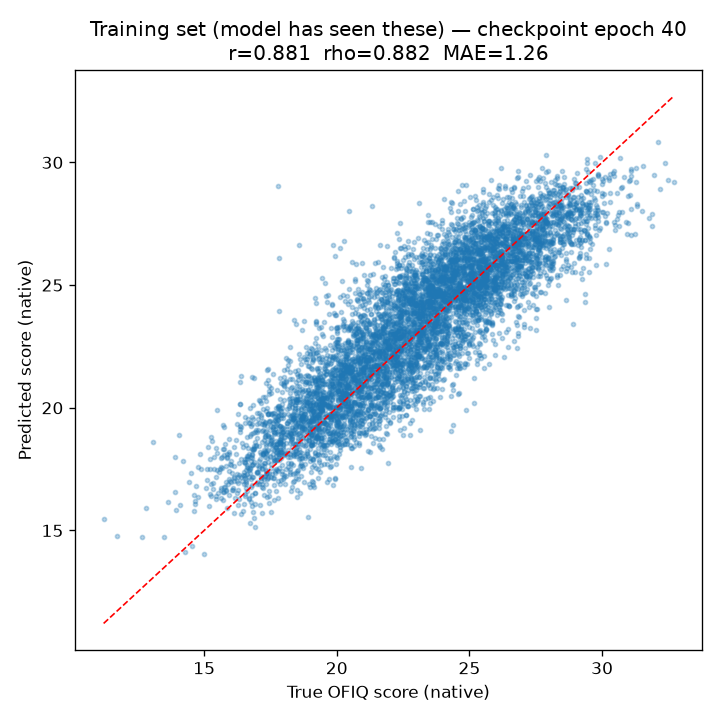
\includegraphics[width=0.88\textwidth]{figures/eval_scatter_full_train.png}
\caption{Predicted versus true scores on training images (dropout off). Comparable tightness to Figure~\ref{fig:scatter_val} indicates the model is not merely memorizing.}
\label{fig:scatter_train}
\end{figure}

\subsection{Example predictions}

Table~\ref{tab:examples} lists twelve held-out examples spaced across the validation list. Most errors lie within $\pm 2$ native points; larger residuals tend to appear near distribution extremes.

\TableHere[14\baselineskip]
\caption{Example held-out predictions (native OFIQ units).}
\label{tab:examples}
\centering
\footnotesize
\begin{tabularx}{\textwidth}{|L{0.34\textwidth}|C{0.14\textwidth}|C{0.14\textwidth}|C{0.14\textwidth}|Y|}
\hline
\textbf{Image} & \textbf{True} & \textbf{Pred.} & \textbf{Error} & \\
\hline
\texttt{ffhq\_all/49936.png} & 23.3 & 25.2 & $+1.9$ & \\
\hline
\texttt{ffhq\_all/04591.png} & 22.4 & 23.1 & $+0.6$ & \\
\hline
\texttt{ffhq\_all/10849.png} & 26.0 & 24.4 & $-1.6$ & \\
\hline
\texttt{ffhq\_all/17289.png} & 17.3 & 19.9 & $+2.6$ & \\
\hline
\texttt{ffhq\_all/64087.png} & 18.8 & 18.9 & $+0.1$ & \\
\hline
\texttt{ffhq\_all/57157.png} & 19.2 & 23.3 & $+4.1$ & \\
\hline
\texttt{ffhq\_all/50969.png} & 21.3 & 20.8 & $-0.6$ & \\
\hline
\texttt{ffhq\_all/44661.png} & 24.5 & 25.2 & $+0.7$ & \\
\hline
\texttt{ffhq\_all/38253.png} & 21.1 & 18.7 & $-2.3$ & \\
\hline
\texttt{ffhq\_all/31335.png} & 25.0 & 25.9 & $+0.9$ & \\
\hline
\texttt{ffhq\_all/25036.png} & 27.3 & 25.1 & $-2.3$ & \\
\hline
\texttt{ffhq\_all/41869.png} & 30.1 & 27.6 & $-2.5$ & \\
\hline
\end{tabularx}
\end{table}

\FloatBarrier
\section{Mapping to Problem-Statement Requirements}
\label{sec:rubric}

This section explicitly maps completed work to rubric items~1--4. Item~5 from broader integration checklists is \textbf{not} claimed as completed work; see Section~\ref{sec:assumption}.

\subsection{Rubric 1 --- Understand the data}

\begin{itemize}[leftmargin=*]
    \item Ground truth identified as OFIQ \texttt{UnifiedQualityScore.native}, not human Likert labels and not the squashed scalar.
    \item Label generation process documented (OFIQ batch over FFHQ; CSV schema; filename join).
    \item Score range, missing-file handling, and leakage-safe split statistics reported (Section~\ref{sec:data}).
\end{itemize}

\subsection{Rubric 2 --- Define the task precisely}

\begin{itemize}[leftmargin=*]
    \item Task fixed as single-score regression with scaled sigmoid output and native unscaling (Section~\ref{sec:task}).
    \item Loss chosen to combine absolute fidelity (MSE) with ranking fidelity (Pearson term).
    \item Success metrics aligned with quality-ranking use (Pearson $r$, Spearman $\rho$, MAE).
\end{itemize}

\subsection{Rubric 3 --- Design a small CNN}

\begin{itemize}[leftmargin=*]
    \item Custom SmallResNet at $\approx 0.33$M parameters replaces an 11M-parameter overfit baseline (Section~\ref{sec:arch}).
    \item Efficiency-motivated choices: few channels, one block per stage, global average pooling, no pretrained dependency for offline nodes.
    \item Regularization appropriate to conv features (Dropout2d, SE, augmentation, AdamW).
\end{itemize}

\subsection{Rubric 4 --- Train and validate}

\begin{itemize}[leftmargin=*]
    \item Reproducible 90/10 split with persisted validation file list.
    \item Full training protocol with early stopping, LR schedule, and gradient clipping (Section~\ref{sec:train}).
    \item Held-out evaluation shows MAE $1.32$, $r=0.866$, $\rho=0.867$, and $\approx 2\times$ improvement over mean baseline (Section~\ref{sec:results}).
    \item Measurement and checkpointing corrected under advisor feedback so reported curves and saved weights are defensible.
\end{itemize}

\FloatBarrier
\section{Assumed Downstream Use in Generative Training}
\label{sec:assumption}

The problem statement situates a face-quality CNN as infrastructure for a larger generative model: once trained, the network (or its representation) can contribute a quality signal to the generator's objective so that synthesized faces are pushed toward higher usability, not only lower pixel error.

\textbf{Assumption (not implemented in this report).} We assume that Spencer's subsequent generative-training pipeline will treat the trained SmallResNet as a \emph{frozen differentiable quality critic} inside a GAN or related generator loop \citep{goodfellow2014gan}. Under that assumption:
\begin{enumerate}[leftmargin=*]
    \item Generator outputs (or reconstructed faces) are resized/normalized exactly as during our evaluation.
    \item The critic is run in evaluation mode (dropout disabled) with \textbf{frozen} weights.
    \item The scalar output is interpreted as \textbf{higher = better} OFIQ-like unified quality in native units after Equation~\eqref{eq:unscale}, or equivalently in scaled $[0,1]$ space before unscaling.
    \item A generator loss term of the form $\lambda\,(1-\hat{z})$ or $-\lambda\,\hat{y}$ (sign depending on scaling) would encourage higher predicted quality; $\lambda$ would be chosen empirically so the critic does not overpower reconstruction/adversarial terms.
\end{enumerate}
This section does \textbf{not} claim that such coupling has been engineered, ablated, or trained end-to-end here. It records the intended research use so that the numeric contract of our model is unambiguous when that work begins.

\FloatBarrier
\section{Limitations and Future Work}
\label{sec:limits}

\begin{itemize}[leftmargin=*]
    \item The model approximates OFIQ, not human preference directly; residual error may reflect OFIQ-hard cases (subtle pose, occlusion, lighting).
    \item Only the unified score is predicted; multi-head prediction of OFIQ components could yield richer generator feedback.
    \item Pearson $r\approx 0.87$ leaves headroom; larger (but still compact) backbones or limited pretraining might help if offline constraints allow.
    \item Image access on shared cluster storage and Drive copies remains an operational bottleneck for new machines.
    \item Assumed GAN integration (Section~\ref{sec:assumption}) requires future engineering: detach/frozen modes, loss weighting, and checks that the critic cannot be trivially fooled by adversarial generator shortcuts.
\end{itemize}

\FloatBarrier
\section{Conclusion}
\label{sec:conclusion}

This project delivers a compact CNN that predicts OFIQ unified face-image quality on FFHQ with strong held-out correlation (Pearson $r=0.866$, Spearman $\rho=0.867$) and low absolute error (MAE $1.32$ native units), while avoiding the severe overfitting observed with ResNet-18. The work satisfies the problem statement's requirements to understand the data, define a regression task, design a small network, and validate generalization. Advisor feedback on checkpoint selection and train-metric logging was incorporated so that reported curves and saved weights are scientifically defensible. Downstream use as a frozen quality term inside generative training is stated as an explicit assumption for later work, not as a completed deliverable.

\clearpage
\bibliography{references}

\end{document}
